\documentclass[conference]{IEEEtran}
\IEEEoverridecommandlockouts
% The preceding line is only needed to identify funding in the first footnote. If that is unneeded, please comment it out.
\usepackage{cite}
\usepackage{amsmath,amssymb,amsfonts}
\usepackage{algorithmic}
\usepackage{graphicx}
\usepackage{textcomp}
\usepackage{xcolor}
\usepackage{float} % Add this in your preamble if not included
\def\BibTeX{{\rm B\kern-.05em{\sc i\kern-.025em b}\kern-.08em
    T\kern-.1667em\lower.7ex\hbox{E}\kern-.125emX}}
\begin{document}

\title{Phase 4 - Literature Survey and Results\\}

\author{
\IEEEauthorblockN{Jason Weeks}  
\IEEEauthorblockA{\textit{Department of Computer Science} \\  
\textit{Mississippi State University} \\  
Starkville, Mississippi, USA \\  
jcw1044@msstate.edu}  
\and  
\IEEEauthorblockN{Andrew McBride}  
\IEEEauthorblockA{\textit{Department of Computer Science} \\  
\textit{Mississippi State University} \\  
Starkville, Mississippi, USA \\  
ahm228@msstate.edu}  
\and
\IEEEauthorblockN{Andrei Roskelley Garcia}  
\IEEEauthorblockA{\textit{Department of Computer Science} \\  
\textit{Mississippi State University} \\  
Starkville, Mississippi, USA \\  
ar2888@msstate.edu} 
\and
\IEEEauthorblockN{Jacquies Turner}  
\IEEEauthorblockA{\textit{Department of Computer Science} \\  
\textit{Mississippi State University} \\  
Starkville, Mississippi, USA \\  
jt2485@msstate.edu}  
}

\maketitle

\section{Introduction}
This paper will present the relevant literature in the process of traffic signal control using machine learning techniques, along with the timeline of research developments over time.  

\section{Taxonomy}

Research on traffic signal methods falls into three categories. These include single agent learning models, multi agent reinforcement learning models (MARL), and large-scale multi-agent learning models, with the large-scale MARL actively having new deep learning models applied in recent research. 

\subsection{Single Agent Learning Models}

Before 2010, traffic prediction models were designed using single agent reinforcement learning models. These models were used to predict the movement of traffic using a single system, meaning a single neural network predicted how traffic lights should function. While innovative, they are generally not scalable for multiple intersections and can more effectively be used to predict how traffic signals function at a single intersection. These models were rarely used in practice and traffic signals used fixed intervals (threshold signaling) \cite{1}. As a result, we will not focus too much on these for our traffic problem. 

\subsection{Multi Agent Learning Models}

From 2010-2018, research began to focus on multi-agent learning reinforcement (MARL) models, a more practical approach to traffic signal control. These use several systems, or agents, to predict traffic flow for traffic signal control more accurately, but tend to be limited to knowledge of their own environment and not nearby intersections \cite{2}.

During this research period, the majority of models used a variation of Q-Learning. While not perfect, there were indications that there were improvements in terms of moving traffic over traditional timer methods. \cite{2} Eventually, a distributed MARL signal was designed such that each agent may learn the environment independently and communicate the signals it received to nearby agents to improve performance. This further came with the benefit of allowing one agent to fail without taking other agents down, increasing reliability and scalability \cite{5}. This innovation led to major improvements that have influenced the modern design of reinforcement learning techniques for traffic signal control. 

\subsection{Large Scale Multi-Agent Learning Models}

Since 2019, research indicates that MARL agents have been improved for scalability, performance, real-world applications and become open-source. The field has seen enormous growth from the initial small scale solutions, and large scale implementations for real world cities continue to become more practical and powerful.

Early breakthroughs in large-scale MARL focused on a more difficult problem: urban traffic management. This initially came with a new open sourced model, CityFlow, a multi-agent reinforcement model which could handle large road networks with thousands of intersections in a simulated environment \cite{7}. These large-scale models have shown significant improvements in performance while working at a larger scale, making them more adaptable to real situations. 

In recent years, strong reinforcement learning models, such as long short-term memory (LSTM) and spatiotemporal graph convolutional neural networks (STGCN) have been applied to research, and external factors like pedestrian movements have begun being addressed. These advancements show more promise in scalability and performance, but are still in progress. There are still opportunities to test different models which may perform better in synchronization with other agents. While accounting for pedestrians marks a major step in optimizing the traffic signal problem, it opens more questions, such as how can we account for emergency vehicles, namely ambulances or police cars, or collisions that disturb the natural flow of traffic. Despite these questions, these models are very powerful in comparison to previous threshold traffic signal management systems. 

\subsection{Taxonomy Figure}

\begin{figure}[H]
    \centering
    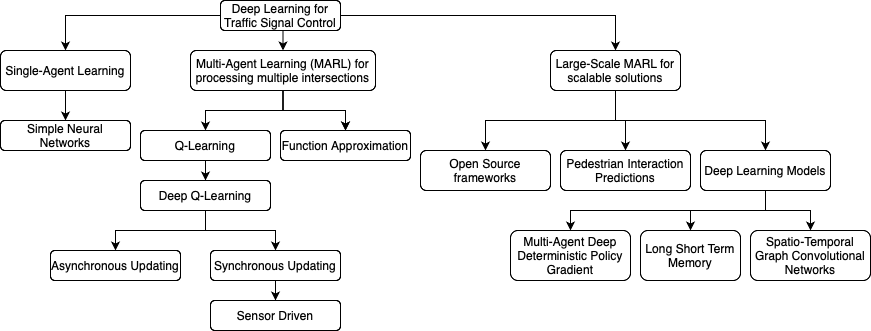
\includegraphics[width=0.9\linewidth]{Research Taxonomy.png}
    \caption{Research Taxonomy for Traffic Signal Control}
\end{figure}


\section{Chronological Overview}
Based on the major research contributions, we have concluded that the papers fall into several categories. These categories tend to reflect the time period of the research contribution, with older papers using less-powerful Q-Learning simulations, and more recent papers using more powerful neural networks with account for more factors. Figure 2 highlights a chronological overview of the categorization of papers over time. 

\begin{figure}[H]
    \centering
    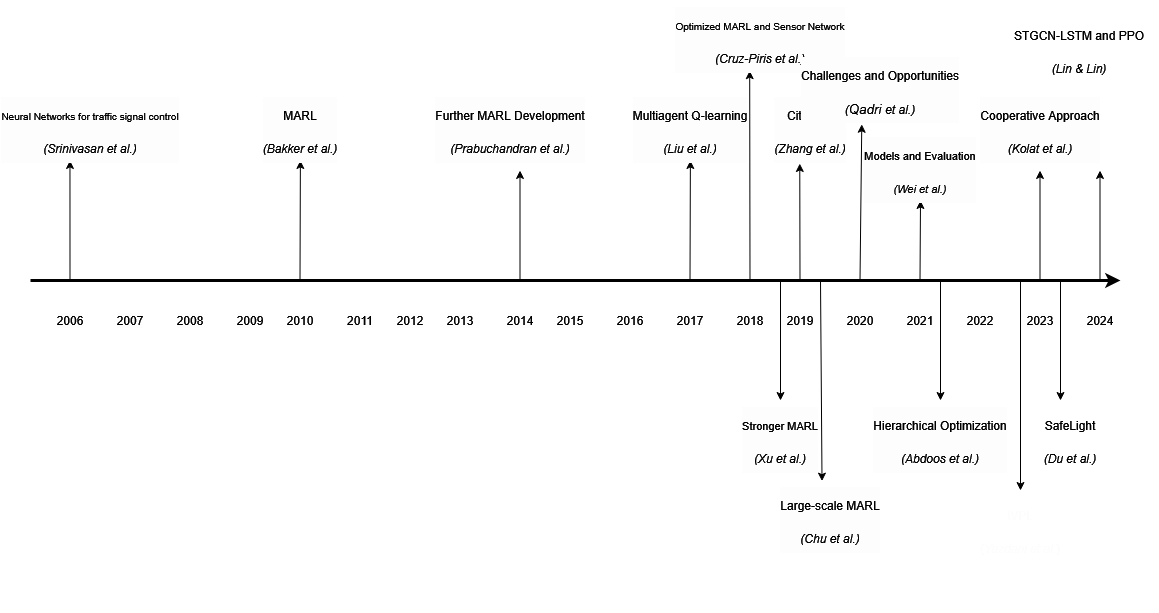
\includegraphics[width=0.9\linewidth]{Diagram Timeline.png}
    \caption{Research Timeline for Traffic Signal Control}
\end{figure}

\section{Research Gaps}
One current research gap is the types of models used. Early MARL models used various Q-learning techniques, with more recent studies using more advanced deep learning techniques, such as LSTM, but transformer-based models and RNN models seem to have been less tested. There are opportunities to test and benchmark different complex deep learning frameworks against each other. 

Another research gap is regards real-world application. Several large cities have adapted deep learning techniques for traffic signal processing, though a large majority of cities do not yet have these technologies implemented. Therefore, they could see a change in performance depending on the size of the city and their road systems. 

A third research gap appears to be the influence of various real-world distractions that can occur, ranging from road accidents, pedestrians, and emergency vehicles. Although Du et al. have begun to take into account pedestrians \cite{13}, there are still several factors that remain unaccounted for in the traffic signal prediction process, which can back up traffic worse than threshold options.

\section*{Work Distribution}
The majority of research findings were made by Jason Weeks and Andrew McBride with help from Andrei by branching out from the original CityFlow paper \cite{7} and finding predecessors and related articles in the field. 

Based on the research findings, Jason Weeks, Jacquies Turner, and Andrew McBride contributed to the research taxonomy and timelines. These were made by narrowing down the most important research articles in our original findings.  

This paper was primarily written by Jason Weeks, but all the members contributed. 

The final distribution of the work is as follows. 

\begin{itemize}
    \item 25\% - Jason Weeks
    \item 25\% - Andrew McBride
    \item 25\% - Jacquies Turner
    \item 25\% - Andrei Roskelley Garcia
\end{itemize}


\section{Simulation Environment and Data Preparation}

To effectively evaluate MARL models for traffic signal control, we will employ CityFlow, a multi-agent traffic simulation engine. CityFlow enables efficient traffic modeling by allowing pre-designed scenarios to be simulated instead of relying on real-time data. This approach provides greater flexibility in the definition and testing of traffic environments, making it ideal for research applications. CityFlow is particularly suited for large-scale urban traffic modeling. By simulating traffic flow in a controlled environment, we can test different reinforcement learning models without disrupting real-world traffic. The engine allows for scalable simulations with thousands of intersections, making it a powerful tool for evaluating various traffic control algorithms. For this study, CityFlow will be used to model the traffic network of Starkville, Mississippi, a city that currently employs traditional timer-based traffic light systems. This provides a relevant testing ground for machine learning-based traffic optimization, as improvements in traffic flow could have tangible real-world benefits.

The dataset used for traffic simulation consists of two primary components: roadnet.json and flow.json. The roadnet.json file defines the city's infrastructure, including the road layout, intersections, lane directions, traffic signals, and turning rules. This data is extracted from OpenStreetMaps (OSM) for Starkville and will be converted into a SUMO network before being integrated into CityFlow. Meanwhile, the flow.json file captures the dynamic movement of vehicles within the network, specifying entry and exit points, common routes, and characteristics such as vehicle priority and speed. Since real-world traffic flow data is not readily available, SUMO tools will be used to generate realistic traffic patterns, ensuring an accurate simulation environment to test reinforcement learning-based traffic control strategies.

Starkville presents an ideal case study due to its unique combination of urban and suburban traffic patterns. Unlike many cities that have adopted sensor-based or pressure plate-based signaling systems, Starkville still relies on traditional timer-based traffic signals, making it a prime candidate for testing reinforcement learning-based optimizations.

\section{Implementation}

Our implementation will involve using CityFlow traffic simulation to estimate how traffic flows in Starkville and customize the minutia to our liking much more efficiently than a tool like SUMO. We can collect data from the environment such as congestion levels and states of other environments, along with a set of possible actions to implement a deep Q-learning model, which will reward or punish our model based on actions taken.

Because deep learning is computationally challenging, we will use a joint model. With this model, every action taken will result in a punishment or reward score for the model as a whole. This will allow us to train only one neural network at a time and comes with the added benefit of rewarding actions based on how they affect the state of other intersections. A model like this has historically proven to be more efficient than existing threshold signaling. Our ultimate goal is to prove that this model can provide better traffic signal decisions than existing threshold systems such as those used in Starkville. 

\section{Importance and Challenges}

Because traffic light timing plays a crucial role in creating frustrated drivers and accidents, it is critical to find the most effective strategy to create smooth traffic flow through traffic signal control. As a result, our plan for the next two months is to implement a MARL model to predict traffic signals for the city of Starkville Mississippi, a city that uses threshold signaling for various times of the day to move traffic. It could be trained to predict various scenarios, including high-intensity traffic after an athletic event or lighter traffic during school breaks, with the ultimate goal of outperforming existing methodologies for traffic signal processing during all times of the day. 

However, there are a variety of challenges with implementation. One challenge is the difficulty in finding optimal Q values as there is no ground truth to compare it to, the agent has to guess and learn on the experience and rewards it receives. This method is also very computationally challenging, as the agent has to constantly update the Q-value, especially with very large and complex models. There is also difficulty in balancing exploration vs exploitation, if the agent explores too much, then the Q-value may not converge to its optimal value, and if it exploits what it knows too much then the value may get stuck at a suboptimal level. Solving this would require understanding and the use of certain exploration strategies. There are also problems that could arise with the environment. The environment can slowly change overtime, so our Q-value may become irrelevant, so the agent would have to relearn its environment. There are also many unexpected situations that may arise that may require the model to quickly learn and adapt in the unknown situation, or try to reinforce the model to account for these situations.

\section{Development plan}

Implementing a traffic simulation for Starkville, MS using CityFlow and Q-Learning over a two-month period, we will begin with the research and environment setup in the first two weeks. This includes installing and configuring CityFlow, generating traffic flows using built-in tools, and setting up a simulation model based on the Starkville road network and intersections. If real-world traffic data is available, we will incorporate it to enhance accuracy; otherwise, default CityFlow scenarios will be used. During weeks three to six, we will develop and train the Q-Learning algorithm by optimizing hyperparameters such as learning rate and exploration rate and running simulations to evaluate its performance. The effectiveness of Q-Learning-controlled signals will be compared against traditional fixed-time signals using metrics like vehicle waiting times and overall traffic flow improvements. In the last two weeks, we will focus on optimizing and validating the model, testing it under different traffic conditions specific to Starkville, Ms. The model will be deployed in a full-scale SUMO simulation, validated against available traffic data, and adjusted accordingly. The project will conclude with documentation of the implementation details and findings, while also identifying opportunities for future improvements, such as deep reinforcement learning for more advanced control. Ultimately, this project aims to develop an intelligent traffic light control system that reduces congestion and improves traffic efficiency in Starkville, Mississippi.

\section{Implemented Application}

\subsection{Simulation Setup}

After starting implementation, we decided that CityFlow was not the appropriate tool for this problem, despite our research. While a powerful tool, it struggled to handle the data format provided from OSM data, resulting in slow performance and broken intersections. We then decided moving to the SUMO simulator was a more worthwhile decision, as its efficiency has improved over time and documentation is more appropriate for our specific research area. 

Once SUMO was installed, we downloaded public data for the city of Starkville Mississippi's road structure using the tool open street map, and used SUMO's netedit to process the data into a usable format. Some changes were made, such as fixing traffic signal placement using junctions and fixing non-signal-based intersection interactions. 

Our ultimate goal with this project is to test how neural network influenced traffic signals direct the flow of traffic, so we needed to setup various simulation environments to simulate realistic traffic scenarios within Starkville. To do this, we used SUMO's built in flow generator, with various parameters to result in light, medium, and intense traffic scenarios. This would allow us to test how each method of traffic signal control reacts to various events such as morning and afternoon rush hours, post game traffic, or light summer traffic. 

Using the configuration file, we can use the SUMO GUI, which comes included with the SUMO installation package. This tools allows us to run a visualization of the simulation with regards to the currently implemented method of traffic signal control, and make observations from the point of view of drivers without quantitative analysis, making observations about our model to make improvements. a

\begin{figure}[H]
    \centering
    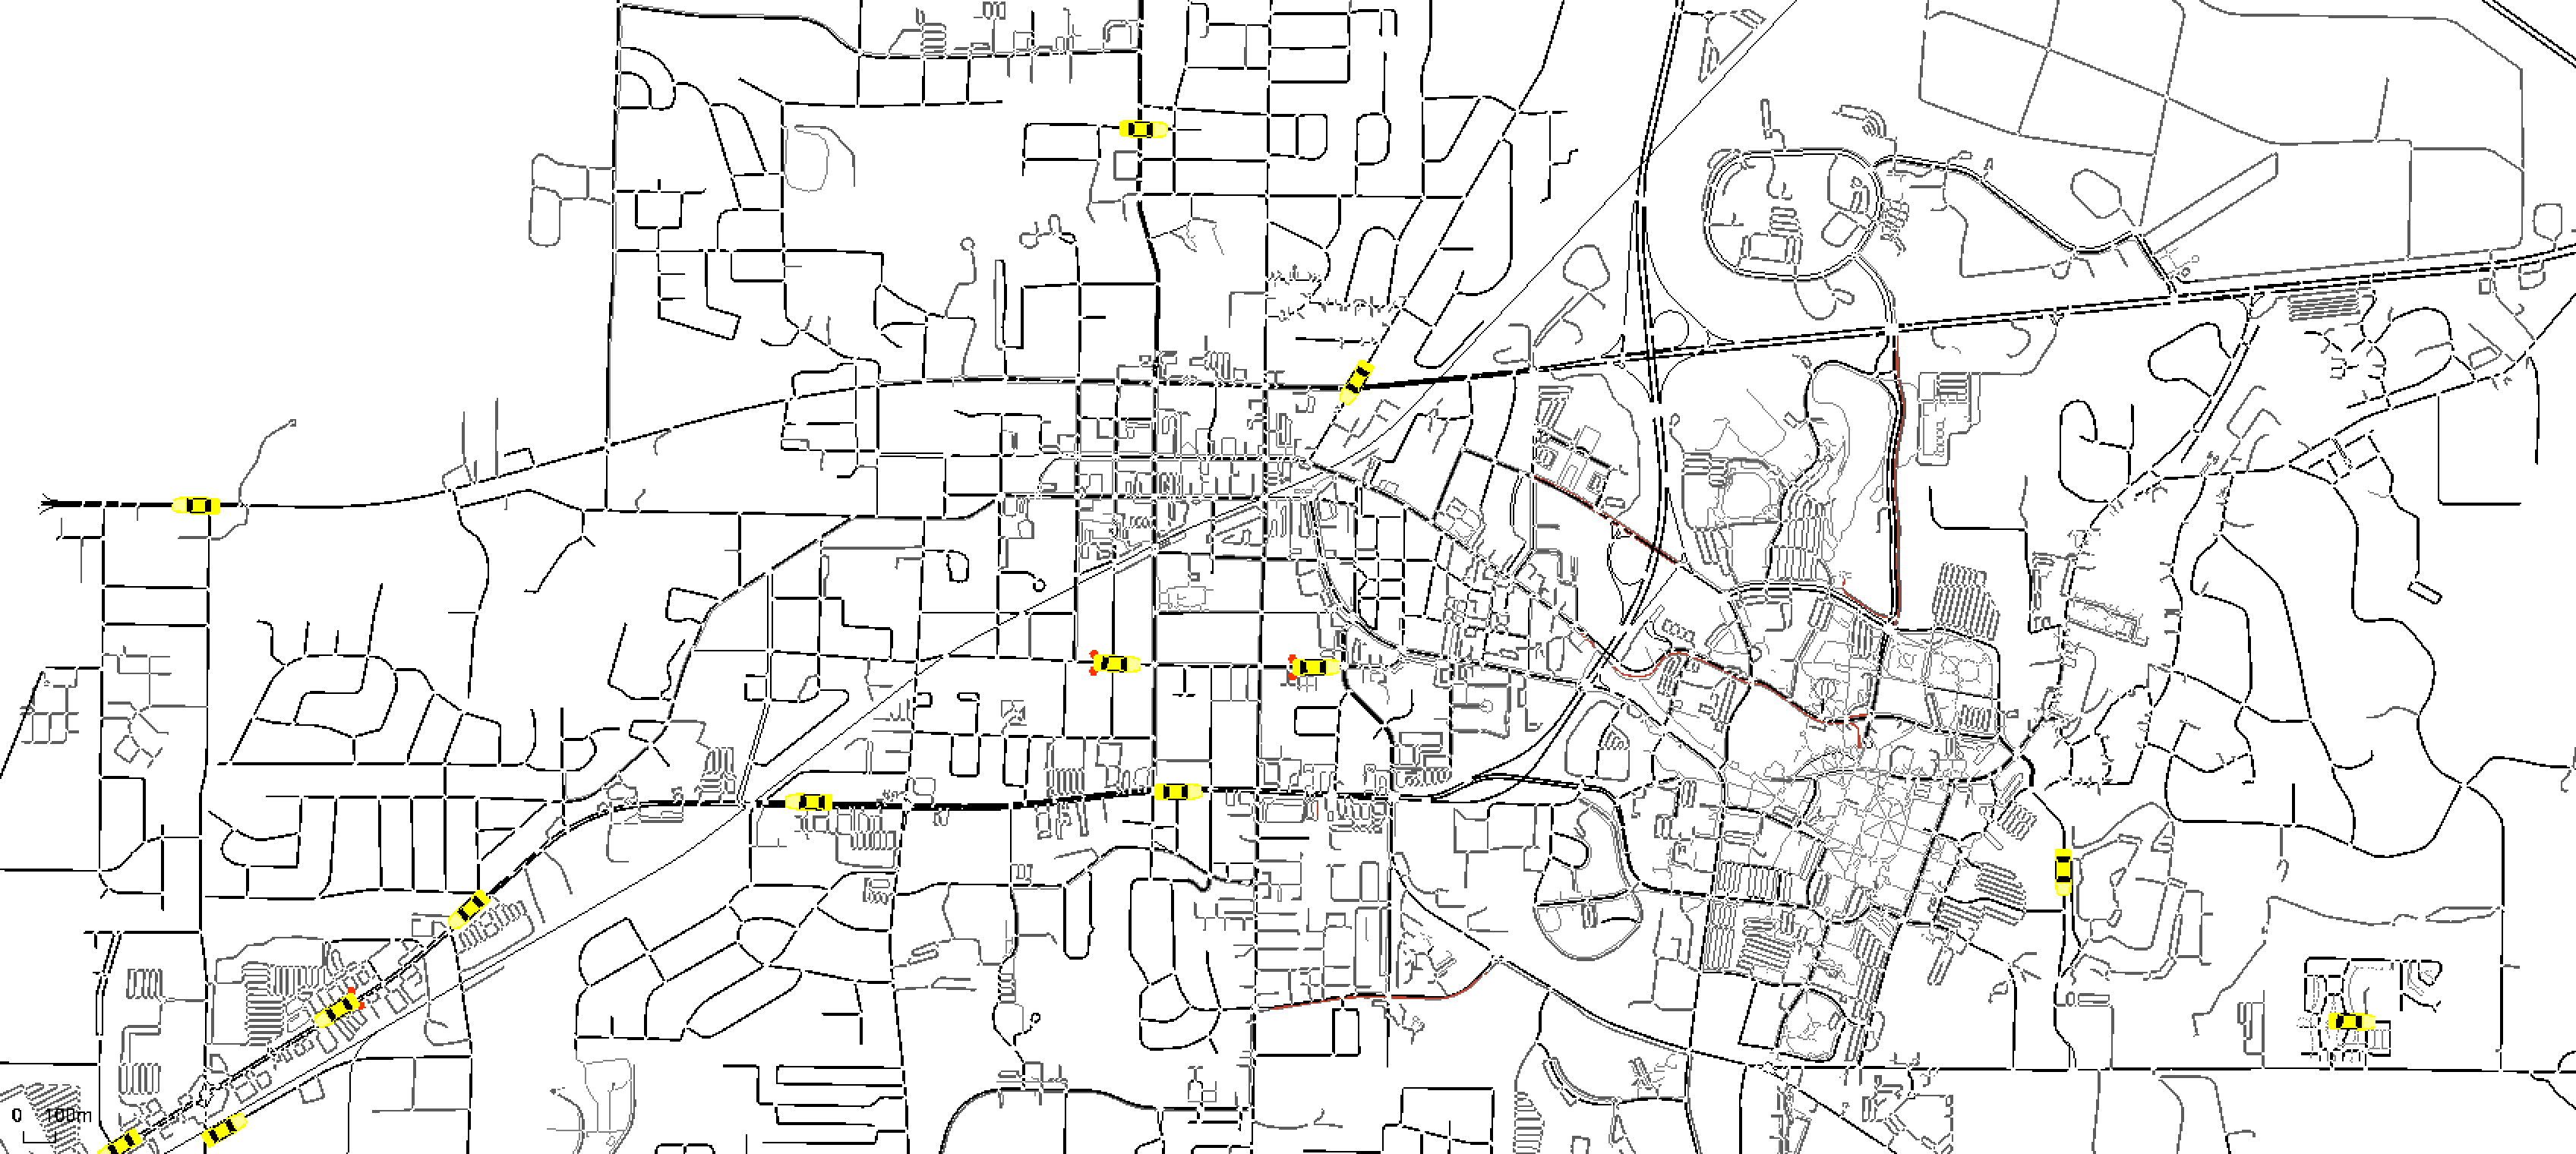
\includegraphics[width=0.9\linewidth]{SUMO_RUNNING.png}
    \caption{Example of SUMO running in through SUMO-GUI}
\end{figure}

\subsection{Benchmarking}

In order to properly evaluate the performance of threshold and neural network models, a method of evaluation was needed beyond qualitative methods, such as observation or review. As a result we implemented various benchmarks to quantitatively decide the quality of a methods approach. 

Our first method of benchmark involves calculating the average waiting time of a vehicle. This is the most likely representation of how frustrated one might feel. A lower waiting time is therefore a great benchmark, as it shows that traffic is moving and drivers are less likely to get frustrated and develop road rage or get into an accident. 

The next is the average trip time. Because we will benchmark similar environments, we can get the average trip times of all combined vehicles in a simulation, and use it as a quantitative performance metric. Faster trips indicate a successful implementation of traffic signal control, as people can get to their end destination faster. It also serves as a benchmark for other metrics, likely indicating shorter queue lengths, less stops, and less time waiting at stops on average. 

Our final benchmark involves calculating queue lengths, or the average length of cars in line at an intersection. We can calculate both the max and average, to ensure the model is acting appropriately and not building super long lines to get the average down. A long line indicates that the model has a lot of buildup, and might fill later intersections with traffic, resulting in frustrated drivers and numerous stops if not carefully considered; therefore, it is critical that we minimize both the average queue length and the max queue length with our neural network. 

Because there are several benchmarks, we will consider our model successful if any evaluation metric improves without a meaningful reducing another metric. For example, if average trip time decreases, but the other metrics remain very similar to their threshold results, we will consider the model a success.

\subsection{Neural Network Implementation}

Our neural network is implemented through the python libraries traffic control interface (traci) and pytorch. Traci allows us to modify our simulation and get state information within a current timestep, while pytorch allows us to easily build and implement neural networks for our project. 

The first step in designing the proposed neural network is to establish what an agent is, and how they will communicate with the model. Based on existing codebases and research, we decided to implement a decentralized multi-agent reinforcement learning model. This specific implementation lacks a central coordinator, and each agent acts on its own in coordination with other agents. The agents were designed to represent an intersection with a traffic signal controller, and could accept the state of the lanes leading to the intersection, the state of the signals, and the states of vehicles at each intersection such as stopped time; it also accepted a list of possible actions the traffic signal controller could perform, which when provided to a deep-q learning model can guess the optimal move.  

After designing an agent we decided to model the simulation environment in python to actually obtain states and actions for each agent. To do this, we used traci to obtain the states of vehicles on the lanes of traffic heading towards a specific traffic light, and assigned them to the traffic light. We then grabbed the possible state of actions, again assigning it to said traffic signal. This is necessary for computing optimal actions later. We gather these every 5 seconds in the simulation, which greatly increases performance, and prevents rapidly switching signals during learning. 

Our initial plan was to predict the optimal states of every intersection with a traffic light in Starkville, MS, however, upon implementation we realized our available hardware and time frame would not allow us to do this. Instead, we opted to only use what we decided were points of interest, or intersections where traffic is particularly backed up. Most of these points were decided by considering the importance of the road, the time spent at intersections, and personal experience. This way we don't waste computational resources at intersections that see little traffic, or do fine directing traffic on their own. Doing so significantly decreases the computational requirements to run the model, and also allows us to focus only on important points. 

Our model does not have preset correct moves, which makes designing a neural network a very difficult task. Therefore, its important to choose a (non supervised), q-score, action, learn. 

implementing benchmarks

\section{Results over baseline}

In order to evaluate our model we did two tests, a qualitative analysis, which involves viewing the simulation to compare the original simulation to the baseline, and quantitative analysis where benchmarks were ran to evaluate the model with numbers representing the time taken driving and length of queues. Both methods are critical to effective analysis of the model. While training involved generating various traffic scenarios, or events where cars start at one point and end at another point, our testing involves one scenario, which uses similar traffic patterns seen to training. Using a single traffic scenario allows us to make observations of threshold and neural network based signals. This ensures that while testing, each vehicle has takes the same route so we can observe how our traffic signal management system performs relative to other methods. 

\subsection{Qualitative Analysis}

When observing the baseline threshold-based traffic signals, it did an acceptable job managing light-medium traffic (2000 vehicles per hour), but saw relative redundancy with lights changing while no cars were in the opposite direction, causing congestion on major roads. It felt familiar, with minor traffic on less congested roads, such as backroads connected to highways and highways without traffic stops, but was certainly not as effective as possible. 

The MARL Deep Q-learning model saw notable improvements in terms of responsiveness. When there was no signs of incoming traffic or lines in stopped lanes, it skipped the redundancy of changing the state of traffic lights resulting in a generally smoother flow of traffic. When it did change, it seemed intelligent, considering how long cars have been waiting along with how many cars were waiting. While our model did not allow collisions to be considered, the more continuous flow of traffic saw less emergency stops, and generally safer roads. Analysis also revealed that vehicles would often arrive at their destination sooner than their threshold counterparts, with less time spent on the road generally resulting in safer roads with less congestion.  

There were some limitations of MARL Deep Q-learning despite its generally better analysis. Oftentimes, a light would not change for long periods of times to direct more intense traffic at the expense of shorter lines. This would generally result in shorter average drive lengths, with one drive taking exceptionally long. This was relatively controlled, however, with no cars getting completely stuck, and eventually being directed even if it took a minute. It was also important to choose the right intersections as points of interest, as intersections with little to no congestion would flip their signals the moment a car came to an intersection. It was generally better for areas with extremely light traffic to stick with threshold signals. For points like these, a potentially better option is sensor based traffic signal controllers, which use more concrete rules to change traffic, but make observations similar to our learning model to inform these decisions. 

\subsection{Quantitative Analysis}

While simple observations provide great insight to the performance of our model, numbers to support our observations are potentially more important. As mentioned earlier, we developed several benchmarks based on the results of a simulation. Each benchmark provides a real insight that indicates the performance of a traffic signal control method without the need to make observations. 

The first benchmark was..

the seconds

fourth

last

\subsection{Analysis of Overall Results}

yadieaisdfj;asdkf

\section{ACKNOWLEDGMENT OF LLM USE}

Large language models were not used in the writing or analytical process of writing this paper. However, it was used exclusively to summarize papers during the initial research process, just to ensure that the paper was suitable for our research needs as an aid to abstracts. Not every paper analyzed was used. 

\section*{Reference Acknowledgment}
References \cite{1} through \cite{15} highlight the most significant contributions to the study of traffic signal control using machine learning techniques. They highlight how the research has progressed over time and should help guide the development of a model for traffic prediction. 

The other sources provide great insight, but might have had a smaller research impact. Despite this, they are still high-quality papers and can be used to help solve our problem. These are still critical to understand the problem at hand, and have a meaningful impact on development of our traffic prediction model. 

\begin{thebibliography}{00}
\bibitem{1} Bakker, B., Whiteson, S., Kester, L., \& Groen, F. C. (2010). Traffic light control by multiagent reinforcement learning systems (pp. 475-510). Springer Berlin Heidelberg.
\bibitem{2} Prabuchandran, K. J., AN, H. K., \& Bhatnagar, S. (2014, October). Multi-agent reinforcement learning for traffic signal control. In 17th International IEEE Conference on Intelligent Transportation Systems (ITSC) (pp. 2529-2534). IEEE.
\bibitem{3} Srinivasan, D., Choy, M. C., \& Cheu, R. L. (2006). Neural networks for real-time traffic signal control. IEEE Transactions on intelligent transportation systems, 7(3), 261-272.
\bibitem{4} Xu, M., An, K., Vu, L. H., Ye, Z., Feng, J., \& Chen, E. (2019). Optimizing multi-agent based urban traffic signal control system. Journal of Intelligent Transportation Systems, 23(4), 357-369.
\bibitem{5} Liu, Y., Liu, L., \& Chen, W. P. (2017, October). Intelligent traffic light control using distributed multi-agent Q learning. In 2017 IEEE 20th international conference on intelligent transportation systems (ITSC) (pp. 1-8). IEEE.
\bibitem{6} Cruz-Piris, L., Rivera, D., Fernandez, S., \& Marsa-Maestre, I. (2018). Optimized sensor network and multi-agent decision support for smart traffic light management. Sensors, 18(2), 435.
\bibitem{7} Zhang, H., Feng, S., Liu, C., Ding, Y., Zhu, Y., Zhou, Z., ... \& Li, Z. (2019, May). Cityflow: A multi-agent reinforcement learning environment for large scale city traffic scenario. In The world wide web conference (pp. 3620-3624).
\bibitem{8} Chu, T., Wang, J., Codecà, L., \& Li, Z. (2019). Multi-agent deep reinforcement learning for large-scale traffic signal control. IEEE transactions on intelligent transportation systems, 21(3), 1086-1095.
\bibitem{9} Qadri, S. S. S. M., Gökçe, M. A., \& Öner, E. (2020). State-of-art review of traffic signal control methods: challenges and opportunities. European transport research review, 12, 1-23.
\bibitem{10} Wei, H., Zheng, G., Gayah, V., \& Li, Z. (2021). Recent advances in reinforcement learning for traffic signal control: A survey of models and evaluation. ACM SIGKDD Explorations Newsletter, 22(2), 12-18.
\bibitem{11} Abdoos, M., \& Bazzan, A. L. (2021). Hierarchical traffic signal optimization using reinforcement learning and traffic prediction with long-short term memory. Expert systems with applications, 171, 114580.
\bibitem{12} Kolat, M., Kővári, B., Bécsi, T., \& Aradi, S. (2023). Multi-agent reinforcement learning for traffic signal control: A cooperative approach. Sustainability, 15(4), 3479.
\bibitem{13} Du, W., Ye, J., Gu, J., Li, J., Wei, H., \& Wang, G. (2023, June). Safelight: A reinforcement learning method toward collision-free traffic signal control. In Proceedings of the AAAI conference on artificial intelligence (Vol. 37, No. 12, pp. 14801-14810).
\bibitem{14} Yazdani, M., Sarvi, M., Bagloee, S. A., Nassir, N., Price, J., \& Parineh, H. (2023). Intelligent vehicle pedestrian light (IVPL): A deep reinforcement learning approach for traffic signal control. Transportation research part C: emerging technologies, 149, 103991.
\bibitem{15} Lin, T., \& Lin, R. (2024). Smart City Traffic Flow and Signal Optimization Using STGCN-LSTM and PPO Algorithms. IEEE Access.
\bibitem{16} Haydari, A., \& Yılmaz, Y. (2020). Deep reinforcement learning for intelligent transportation systems: A survey. IEEE Transactions on Intelligent Transportation Systems, 23(1), 11-32.
\bibitem{17} Wei, H., Xu, N., Zhang, H., Zheng, G., Zang, X., Chen, C., ... \& Li, Z. (2019, November). Colight: Learning network-level cooperation for traffic signal control. In Proceedings of the 28th ACM international conference on information and knowledge management (pp. 1913-1922).
\bibitem{18} Chen, C., Wei, H., Xu, N., Zheng, G., Yang, M., Xiong, Y., ... \& Li, Z. (2020, April). Toward a thousand lights: Decentralized deep reinforcement learning for large-scale traffic signal control. In Proceedings of the AAAI conference on artificial intelligence (Vol. 34, No. 04, pp. 3414-3421).
\bibitem{19} Zheng, G., Xiong, Y., Zang, X., Feng, J., Wei, H., Zhang, H., ... \& Li, Z. (2019, November). Learning phase competition for traffic signal control. In Proceedings of the 28th ACM international conference on information and knowledge management (pp. 1963-1972).
\bibitem{20} Wei, H., Zheng, G., Gayah, V., \& Li, Z. (2019). A survey on traffic signal control methods. arXiv preprint arXiv:1904.08117.
\bibitem{21} Wei, H., Zheng, G., Yao, H., \& Li, Z. (2018, July). Intellilight: A reinforcement learning approach for intelligent traffic light control. In Proceedings of the 24th ACM SIGKDD international conference on knowledge discovery \& data mining (pp. 2496-2505).
\bibitem{22} Yang, L., Luo, P., Change Loy, C., \& Tang, X. (2015). A large-scale car dataset for fine-grained categorization and verification. In Proceedings of the IEEE conference on computer vision and pattern recognition (pp. 3973-3981).
\bibitem{23} Milan, A. (2016). MOT16: A benchmark for multi-object tracking. arXiv preprint arXiv:1603.00831.
\bibitem{24} Mao, F., Li, Z., \& Li, L. (2022). A comparison of deep reinforcement learning models for isolated traffic signal control. IEEE Intelligent Transportation Systems Magazine, 15(1), 160-180.
\bibitem{25} Noaeen, M., Naik, A., Goodman, L., Crebo, J., Abrar, T., Abad, Z. S. H., ... \& Far, B. (2022). Reinforcement learning in urban network traffic signal control: A systematic literature review. Expert Systems with Applications, 199, 116830.
\bibitem{26} Claus, C., \& Boutilier, C. (1998). The dynamics of reinforcement learning in cooperative multiagent systems. AAAI/IAAI, 1998(746-752), 2.
\bibitem{27} Arel, I., Liu, C., Urbanik, T., \& Kohls, A. G. (2010). Reinforcement learning-based multi-agent system for network traffic signal control. IET Intelligent Transport Systems, 4(2), 128-135.
\bibitem{28} Jácome, L., Benavides, L., Jara, D., Riofrio, G., Alvarado, F., \& Pesantez, M. (2018, October). A survey on intelligent traffic lights. In 2018 IEEE International Conference on Automation/XXIII Congress of the Chilean Association of Automatic Control (ICA-ACCA) (pp. 1-6). IEEE.
\bibitem{29} Mei, H., Lei, X., Da, L., Shi, B., \& Wei, H. (2024). Libsignal: an open library for traffic signal control. Machine Learning, 113(8), 5235-5271.
\bibitem{30} Eom, M., \& Kim, B. I. (2020). The traffic signal control problem for intersections: a review. European transport research review, 12, 1-20.
\bibitem{31} El-Tantawy, S., \& Abdulhai, B. (2010, September). An agent-based learning towards decentralized and coordinated traffic signal control. In 13th International IEEE conference on intelligent transportation systems (pp. 665-670). IEEE.
\bibitem{32} Tang, Z., Naphade, M., Liu, M. Y., Yang, X., Birchfield, S., Wang, S., ... \& Hwang, J. N. (2019). Cityflow: A city-scale benchmark for multi-target multi-camera vehicle tracking and re-identification. In Proceedings of the IEEE/CVF Conference on Computer Vision and Pattern Recognition (pp. 8797-8806).
\bibitem{33} Cools, S. B., Gershenson, C., \& D’Hooghe, B. (2013). Self-organizing traffic lights: A realistic simulation. Advances in applied self-organizing systems, 45-55.
\bibitem{34} Bouktif, S., Cheniki, A., Ouni, A., \& El-Sayed, H. (2023). Deep reinforcement learning for traffic signal control with consistent state and reward design approach. Knowledge-Based Systems, 267, 110440.
\bibitem{35} Ducrocq, R., \& Farhi, N. (2023). Deep reinforcement Q-learning for intelligent traffic signal control with partial detection. International journal of intelligent transportation systems research, 21(1), 192-206.
\bibitem{36} Wang, X., Ke, L., Qiao, Z., \& Chai, X. (2020). Large-scale traffic signal control using a novel multiagent reinforcement learning. IEEE transactions on cybernetics, 51(1), 174-187.
\bibitem{37} Wei, H., Chen, C., Zheng, G., Wu, K., Gayah, V., Xu, K., \& Li, Z. (2019, July). Presslight: Learning max pressure control to coordinate traffic signals in arterial network. In Proceedings of the 25th ACM SIGKDD international conference on knowledge discovery \& data mining (pp. 1290-1298).
\bibitem{38} Zang, X., Yao, H., Zheng, G., Xu, N., Xu, K., \& Li, Z. (2020, April). Metalight: Value-based meta-reinforcement learning for traffic signal control. In Proceedings of the AAAI conference on artificial intelligence (Vol. 34, No. 01, pp. 1153-1160).
\bibitem{39} Zhang, H., Liu, C., Zhang, W., Zheng, G., \& Yu, Y. (2020, October). Generalight: Improving environment generalization of traffic signal control via meta reinforcement learning. In Proceedings of the 29th ACM international conference on information \& knowledge management (pp. 1783-1792).
\bibitem{40} Navarro-Espinoza, A., López-Bonilla, O. R., García-Guerrero, E. E., Tlelo-Cuautle, E., López-Mancilla, D., Hernández-Mejía, C., \& Inzunza-González, E. (2022). Traffic flow prediction for smart traffic lights using machine learning algorithms. Technologies, 10(1), 5.
\bibitem{41} Natafgi, M. B., Osman, M., Haidar, A. S., \& Hamandi, L. (2018, November). Smart traffic light system using machine learning. In 2018 IEEE International Multidisciplinary Conference on Engineering Technology (IMCET) (pp. 1-6). IEEE.
\bibitem{42} Behrendt, K., Novak, L., \& Botros, R. (2017, May). A deep learning approach to traffic lights: Detection, tracking, and classification. In 2017 IEEE International Conference on Robotics and Automation (ICRA) (pp. 1370-1377). IEEE.
\bibitem{43} Ottom, M. A., \& Al-Omari, A. (2023). An adaptive traffic lights system using machine learning. Int. Arab J. Inf. Technol., 20(3), 407-418.
\bibitem{44} Kumar, N., Mittal, S., Garg, V., \& Kumar, N. (2021). Deep reinforcement learning-based traffic light scheduling framework for SDN-enabled smart transportation system. IEEE Transactions on Intelligent Transportation Systems, 23(3), 2411-2421.
\bibitem{45} Sagiroglu, S., Yavanoglu, U., \& Guven, E. N. (2007, December). Web based machine learning for language identification and translation. In Sixth International Conference on Machine Learning and Applications (ICMLA 2007) (pp. 280-285). IEEE.
\bibitem{46} Li, Y., Zhang, Y., Li, X., \& Sun, C. (2024). Regional multi-agent cooperative reinforcement learning for city-level traffic grid signal control. IEEE/CAA Journal of Automatica Sinica, 11(9), 1987-1998.
\bibitem{47} Peng, X., Gao, H., Han, G., Wang, H., \& Zhang, M. (2023). Joint Optimization of Traffic Signal Control and Vehicle Routing in Signalized Road Networks using Multi-Agent Deep Reinforcement Learning. arXiv preprint arXiv:2310.10856.
\bibitem{48} Zhang, Y., Yu, Z., Zhang, J., Wang, L., Luan, T. H., Guo, B., \& Yuen, C. (2023). Learning Decentralized Traffic Signal Controllers with Multi-Agent Graph Reinforcement Learning. IEEE Transactions on Mobile Computing.
\bibitem{49} Wang, K., Shen, Z., Lei, Z., \& Zhang, T. (2024). Towards Multi-agent Reinforcement Learning based Traffic Signal Control through Spatio-temporal Hypergraphs. arXiv preprint arXiv:2404.11014.
\bibitem{50} Chen, F., Chen, Z., Biswas, S., Lei, S., Ramakrishnan, N., \& Lu, C. T. (2020, November). Graph convolutional networks with kalman filtering for traffic prediction. In Proceedings of the 28th international conference on advances in geographic information systems (pp. 135-138).
\bibitem{51} Li, Z., Xu, C., \& Zhang, G. (2021). A deep reinforcement learning approach for traffic signal control optimization. arXiv preprint arXiv:2107.06115.
\bibitem{52} Zhang, Y., Zheng, G., Liu, Z., Li, Q., \& Zeng, H. (2024). MARLens: understanding multi-agent reinforcement learning for traffic signal control via visual analytics. IEEE transactions on visualization and computer graphics.
\end{thebibliography}

\end{document}
